% !TEX options=-shell-escape
\documentclass[12pt]{article}
\usepackage{amsfonts}
\usepackage{amsmath}
\usepackage{siunitx}
\usepackage{fancyvrb}
\usepackage{hyperref}
\usepackage{makecell}
\usepackage[a4paper, total={7in, 10in}]{geometry}
\usepackage{tikz}
\usepackage{footnote}
\usepackage{subcaption}
\usepackage{graphicx}
\usepackage{libertine}
\usepackage{minted}
\usepackage[nottoc]{tocbibind}
\usepackage{tablefootnote}
\usepackage[UTF8]{ctex}
\usepackage{soul}
\usepackage{datetime}

\newdateformat{chinesedate}{\THEYEAR 年\THEMONTH 月\THEDAY 日}

\makesavenoteenv{tabular}
\makesavenoteenv{table}

\definecolor{bg}{rgb}{0.95,0.95,0.95}
\setminted{
  fontsize=\footnotesize,
  bgcolor=bg,
  frame=leftline
}

\providecommand{\keywords}[1]{\small\textbf{\textit{Keywords---}} #1}

\date{2020年9月11日}

\title{多功能Hamilton力学模拟器与其应用案例}
\author{詹有丘}

\begin{document}

\maketitle

\begin{abstract}
我开发了一个可以便捷地模拟Hamilton力学系统的在线软件.
只要用户把系统的Hamiltonian和初始条件告诉模拟器,就能在屏幕上直观地看到这一系统的运动.
该模拟器还能用FFT算法得到运动的频域,进而分析振子的振动模式.
它还能输出被模拟的系统的数据来创建数据集,可用于其他潜在的用途.
模拟器体积小而速度快,
且用户界面相当简单(图形界面用于简单的基础操作,控制台界面用于其他操作),
能方便地对它进行操作以及自定义.
\end{abstract}

\keywords{hamiltonian,模拟,力学,可视化}

\tableofcontents

\section{引入}
\label{sec:intro}

理论力学是很难学习的科目.
人们经常发现自己很难想象力学系统是什么样的,
从而可能想要看看运动的图像.
力学系统被定义之后,能够输出系统的运动的软件被称为力学模拟器.

目前互联网上有不少现存的力学模拟器,
但它们大多存在以下某一项或几项缺点:
\begin{enumerate}
  \item 太庞大.
  有些模拟器非常强大,但代价就是它巨大的体积.
  这使得它们不便携.

  \item 不够方便.
  大多数模拟器要求用户将程序文件下载到磁盘.
  这很不方便,因为当用户换了一台设备时,就需要重新安装软件.

  \item 不够可自定义.
  有些模拟器关注于真实生活中的寻常模型.
  对于刚体接触的问题,它们可能很有用.
  但是它们通常不带有诸如模拟任意有心力场中的运动或解决狭义相对论问题的功能.

  \item 无法输出数据.
  有些模拟器专注于当系统变化时将其呈现出来,
  但它们缺少方便的接口来输出系统运动的数据.

  \item 太难操作.
  有些强大的模拟器具有非常复杂的用户界面,
  这要求用户花费数小时的学习来学会操作模拟器和获取结果.
  这对于新用户非常不友好.
\end{enumerate}

所以,我想要创造一个能解决上述问题的模拟器.
为了使它便于使用,应当把它挂载在一个网页上,
这样任何拥有浏览器的用户只要能访问互联网,就都能使用它.

有了这样一个模拟器,人们就可以更方便地学习理论力学.
通过它,可以对特定的力学系统拥有更感性的认知.
利用这个特性,该模拟器还能用于在物理教育或讲座上呈现动态演示,
在疫情大环境和网络教学飞速普及的时代背景下,这款模拟器将会具有一个非常广阔的应用空间.

\section{符号列表}

注意,如果一个符号具有定义域$A\rightarrow B$,
这意味着它是一个从集合$A$到集合$B$的函数,
那么它有时可以表达该函数的值(在集合$B$中).
即,如果$f:A\rightarrow B$是关于$x$的函数,
那么$f$可以是$f\left(x\right)$的简记.

我们总是假设我们遇到的函数具有足够好的性质,如果我们需要使用这一性质的话.

符号列表由表 \ref{tab:symbols} 给出.
数学运算列表由表 \ref{tab:operations} 给出.

所有的量都在计算机程序中以浮点数实现,
这些量并不需要使用和现实中常用的单位相同的单位,
而是使用其他更加方便的单位(如像素或帧),
所以单位并没有在表中被提到.

有一些模型有特定的符号,在节 \ref{sec:program} 中被提到.
它们并没有被包含在符号列表中,但它们的特别含义在那节中被解释了.

\begin{table}[h]
  \caption{符号列表}
  \label{tab:symbols}
  \centering
  \begin{tabular}{cccc}
    符号 & 定义域 & 意义 & 值\\
    \hline
    $t$ & $\mathbb R$ & 时间\\
    $\Delta t$ & $\mathbb R^+$ & ODE求解器的步长 & $\SI{5e-4}{}$\\
    $\iota$ & $\left\{2\zeta\middle|\zeta\in\mathbb Z^+\right\}$ & ODE求解器中向量的维数\\
    $\mathbf x$ & $\mathbb R\rightarrow\mathbb R^\iota$ & 系统的状态,关于$t$ & $\left(\mathbf q,\mathbf p\right)$\\
    $\mathbf q$ & $\mathbb R\rightarrow\mathbb R^{\iota/2}$ & 广义坐标,关于$t$\\
    $\mathbf p$ & $\mathbb R\rightarrow\mathbb R^{\iota/2}$ & 广义动量,关于$t$\\
    $\mathcal H$ & $\mathbb R\times\mathbb R^\iota\rightarrow\mathbb R$ & Hamiltonian,关于$\left(t,\mathbf x\right)$\\
    $\boldsymbol\omega$ & $\mathbb R^{\iota\times\iota}$ & 用于求辛梯度的矩阵 & $\left[\begin{matrix}
      \mathbf O & \mathbf I_{\iota/2}\\
      -\mathbf I_{\iota/2} & \mathbf O
    \end{matrix}\right]$\\
    $\xi$ & $\mathbb R$ & 画布上的横坐标,以像素为单位\\
    $\eta$ & $\mathbb R$ & 画布上的纵坐标,以像素为单位\\
    $m_t$ & $\mathbb R\rightarrow\mathbb R$ & 从真实的$t$到画布上的$\xi$坐标的映射\\
    $m_y$ & $\mathbb R\rightarrow\mathbb R$ & 从真实的$\mathbf x$分量到画布上的$\eta$坐标的映射\\
    $w$ & $\mathbb Z^+$ & 画面的宽度 & $1024$\\
    $h$ & $\mathbb Z^+$ & 画面的高度 & $768$\\
    $y$ & $\mathbb R$ & $\mathbf x$被绘制的分量\\
    $N$ & $\mathbb Z^+$ & 用于计算DFT的样本数 & $\SI{1e5}{}$\\
    $W$ & $\left[0,1\right)\rightarrow\mathbb R$ & 窗函数 & 见式 \ref{eq:hamming}
  \end{tabular}
\end{table}

\begin{table}[h]
  \caption{运算列表}
  \label{tab:operations}
  \centering
  \begin{tabular}{ccc}
    符号 & 名称 & 定义\\
    \hline
    $\dot f$ & $f$关于$t$的全导数\tablefootnote{
      \label{fn:complete}全导数意味着:
      若$f$是关于$g$的函数, $g$是关于$t$的函数,
      那么$\dot f$是$\frac{\mathrm d}{\mathrm dt}f\left(g\left(t\right)\right)$.
    } & $\frac{\mathrm df}{\mathrm dt}$\\
    $\Delta f$ & $f$的全变化\tablefootnote{
      全变化类似于全导数.见脚注 \ref{fn:complete}. 
    },当$t$变为$t+\Delta t$ & $f\left(t+\Delta t\right)-f\left(t\right)$\\
    $\sum_j^nr_j$ & $n$个关于下标$j$\tablefootnote{
      按计算机中的习惯,下标从$0$开始,而不是$1$.
      这一习惯在本文中被遵守.
    }的数之和 & $\sum_{j=0}^{n-1}r_j$\\
    $\zeta\mathbin\%\chi$\tablefootnote{
      这一记法来自计算机的习惯.
    } & $\zeta$除以$\chi$的余数 & $\zeta-\chi\left\lfloor\frac\zeta\chi\right\rfloor$
  \end{tabular}
\end{table}

\section{物理理论}
\label{sec:theory}

\subsection{动力学预测}

一个动力系统的运动可以用形式为
\begin{equation}
  \dot{\mathbf x}=\mathbf f\left(t,\mathbf x\right)
  \label{eq:ode}
\end{equation}
的常微分方程(ODE)预测,其中$\mathbf f:\mathbb R\times\mathbb R^\iota\mapsto\mathbb R^\iota$
是一个与系统本身有关的特定函数,
$\iota$是某个正整数,
它不必是系统的自由度(DOF) (在我们的情形中,它实际上是DOF的两倍).

\subsection{ODE求解器}
\label{sec:ode_solver}

\VerbatimFootnotes
该ODE (式 \ref{eq:ode})能用Runge--Kutta方法\footnote{
  该算法能用Ruby编程语言更简洁地描述:
  \begin{minted}{ruby}
  dx = b.zip(a).each_with_object([]).sum do |(bj, aj), ary|
    bj * ary.push(f.(t+aj.sum*dt, x+aj.zip(ary).sum{_1*_2}*dt)).last
  end * dt
  \end{minted}
}

\begin{equation}
  \Delta\mathbf x\approx\Delta t\sum_j^sb_j\mathbf K_j,
\end{equation}
被数值求解,其中$\mathbf K_j$被递推地定义为\cite[p. 907]{press2007numerical}
\begin{equation}
  \mathbf K_j:=f\left(t+\Delta t\sum_k^ja_{j,k},\mathbf x+\Delta t\sum_k^ja_{j,k}\mathbf K_k\right).
\end{equation}
$\Delta t$越小,求解器就越精确而低效.

阶数$s$和系数$b_j$与$a_{j,k}$
是不同的Runge--Kutta方法特有的.
这里, 3/8准则\cite[p. 138]{hairer2008solvingODE}被采用.
它的系数在表 \ref{tab:3/8-rule} 中展示.

\begin{table}[h]
  \caption{Runge--Kutta方法3/8准则的系数}
  \label{tab:3/8-rule}
  \centering
  \begin{tabular}{c|cccc|c}
    & \multicolumn{4}{c|}{$a_{j,k}$} & $b_j$\\
    \hline
    \diaghead{\theadfont DiagDia}{$j$}{$k$} & $0$ & $1$ & $2$ & $3$\\
    \hline
    $0$ &        &      &     & & $1/6$\\
    $1$ & $1/3$  &      &     & & $1/3$\\
    $2$ & $-1/3$ & $1$  &     & & $1/3$\\
    $3$ & $1$    & $-1$ & $1$ & & $1/8$
  \end{tabular}
\end{table}

ODE求解器应当保存$t$和$\mathbf x$,
而且每当它前进一步,记录$\left(t,\mathbf x\right)$,
并令$\mathbf x\leftarrow\mathbf x+\Delta\mathbf x$,且$t\leftarrow t+\Delta t$.

ODE求解器能给出任意$t$处$\mathbf x$的数值,
只要$\mathbf f$的数值形式和初值$\mathbf x\left(0\right)$
被给定.

\subsection{构建ODE}

仅有ODE求解器的话,对模拟动力学系统没有帮助.
ODE本身是必须的.
根据物理理论,
有很多构建动力学系统的ODE的方法.
本文采用Hamiltonion方法.

Hamilton力学认为,对于某个动力学系统,存在函数
$\mathcal H:\mathbb R^\iota\times\mathbb R\rightarrow\mathbb R:\left(t,\mathbf x\right)\mapsto\mathcal H\left(t,\mathbf x\right)$
使得该系统的运动满足被称为\textbf{正则方程}\footnote{
  正则方程通常在其他书\cite{hand2008mechanics}\cite[p. 65]{arnold1989mathmech}\cite[p. 132]{landau1976mechanics}中记作
  \begin{equation*}
    \dot{\mathbf q}=\frac{\partial\mathcal H}{\partial\mathbf p},
    \quad
    \dot{\mathbf p}=-\frac{\partial\mathcal H}{\partial\mathbf q}.
  \end{equation*}
}的方程
\begin{equation}
  \dot{\mathbf x}=\boldsymbol\omega\nabla_{\mathbf x}\mathcal H,
\end{equation}
其中$\boldsymbol\omega\nabla_{\mathbf x}$是关于$\mathbf x$的\textbf{辛梯度}.

在Hamiltonian力学的情形下,
矢量$\mathbf x\in\mathbb R^\iota$可以被拆分为两个矢量
$\mathbf q\in\mathbb R^{\iota/2}$和$\mathbf p\in\mathbb R^{\iota/2}$,
分别被称为系统的\textbf{广义坐标}和\textbf{广义动量},
所以$\mathbf x$的分量可以被叫做\mintinline{js}{q0}, \mintinline{js}{q1}, \mintinline{js}{p0}, \mintinline{js}{p1},等等.

因为梯度$\nabla_{\mathbf x}\mathcal H$可以容易地被数值计算,根据
\begin{equation}
  \mathbf f\left(t,\mathbf x\right):=\boldsymbol\omega\nabla_{\mathbf x}\mathcal H,
  \label{eq:def_f}
\end{equation}
我们可以给出式 \ref{eq:ode} 中$\mathbf f$的数值形式,
从而根据节 \ref{sec:ode_solver} 中描述的方法数值求解式 \ref{eq:ode}.

\subsection{分析运动的频域}
\label{sec:theory_fft}

当我们研究动力学系统的周期运动时,
通常会研究它的频域.
所以,我们想要让模拟器具备
展示运动的Fourier变换(FT)
(在一段时间$\left[0,N\Delta t\right)$上的)的能力.
由于我们数值地完成这件事,而且$t$实际上是离散的,
所以我们实际上计算的是离散Fourier变换(DFT).

在节 \ref{sec:fft} 中提到的FFT库提供了计算DFT的方法.
虽然我们可以直接挑一个足够长的区间来计算它的DFT,
但这一操作会导致一些频域中的损失\cite{harris1978ft}.
所以在计算DFT之前,应当在该区间上给运动应用一个窗函数.

有各种窗函数可以选择,
每一种都有它特有的应用场景.
本模拟器默认使用Hamming窗\cite{harris1978ft}
\begin{equation}
  W\left(\zeta\right):=\frac{25}{46}-\frac{21}{46}\cos\left(2\pi\zeta\right),
  \label{eq:hamming}
\end{equation}
因为它适合大多数情况.

\begin{figure}[h]
  \centering
  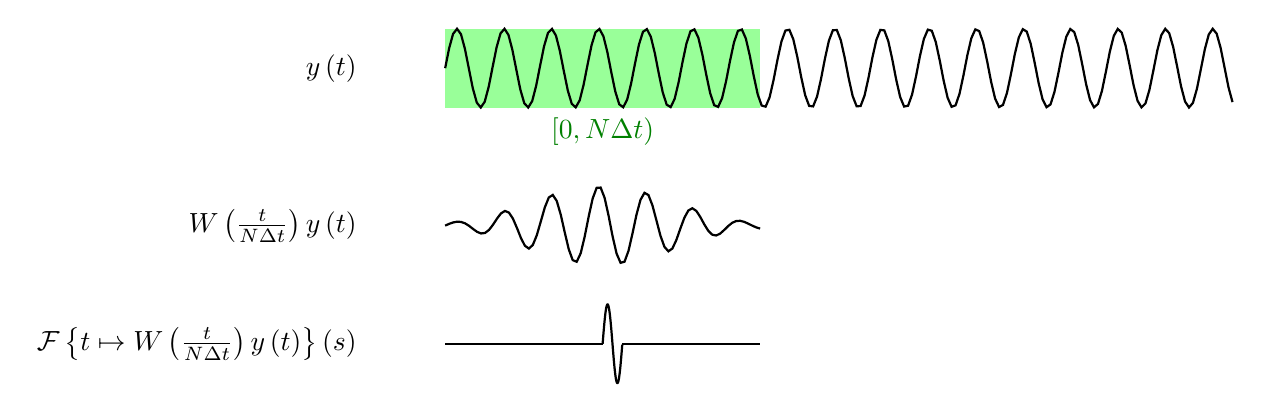
\begin{tikzpicture}
    \node[left] at (-1,-1) {$y\left(t\right)$};
    \fill[green!40!white] (0,-0.5) rectangle +(4,-1);
    \node[below,text=green!50!black] at (2,-1.5) {$\left[0,N\Delta t\right)$};
    \draw[thick,domain=0:10,samples=200,variable=\x] plot ({\x},{0.5*sin(600*\x)-1});
    \node[left] at (-1,-3) {$W\left(\frac t{N\Delta t}\right)y\left(t\right)$};
    \draw[thick,domain=0:4,samples=80,variable=\x] plot ({\x},{(25/46-21/46*cos(360*\x/4))*0.5*sin(600*\x)-3});
    \node[left] at (-1,-4.5) {$\mathcal F\left\{t\mapsto W\left(\frac t{N\Delta t}\right)y\left(t\right)\right\}\left(s\right)$};
    \draw[thick,domain=2:2.25,samples=200,variable=\x] plot ({\x},{0.5*sin(1440*\x)-4.5});
    \draw[thick] (0,-4.5) -- (2,-4.5);
    \draw[thick] (2.25,-4.5) -- (4,-4.5);
  \end{tikzpicture}
  \caption{获取频域的过程}
  \label{fig:fft}
\end{figure}

\section{模拟器使用的库}

该模拟器依赖于一些第三方库.

图形库用于在屏幕上显示图像.

FFT库用于计算系统运动的DFT.

ODE构建器和ODE求解器是我写的,
不依赖第三方库.
它们的理论基础在节 \ref{sec:theory} 中做解释.

\subsection{图形库}

该模拟器使用rpg\_core.js来绘制和显示图像.
这是一个基于 \href{https://www.pixijs.com}{PixiJS} 的网页游戏引擎.
虽然rpg\_core.js附属于非免费的软件 \href{https://tkool.jp/mv}{RPG Maker MV},
但它在 \href{https://github.com/rpgtkoolmv/corescript}{GitHub} 上开源.

在rpg\_core.js中, \mintinline{js}{Bitmap}对象用于存储一幅图片的信息,
而\mintinline{js}{Sprite}对象用于呈现被\mintinline{js}{Bitmap}对象描述的图片.
坐标等信息也在\mintinline{js}{Sprite}对象中\cite{rmmvhelp}.
图 \ref{fig:show_picture} 展示了rpg\_core.js如何显示图片.

\begin{figure}[h]
  \centering
  \begin{tikzpicture}
    \draw (0,0) rectangle +(6,-6);
    \node[below] at (3,-6) {屏幕};
    \draw[thick,->] (0,0) -- +(3,0) node[anchor=south west] {$\xi$};
    \draw[thick,->] (0,0) -- +(0,-3) node[anchor=north east] {$\eta$};
    \shade[inner color=blue,outer color=red] (3,-3) rectangle +(2,-2);
    \node[above left] at (3,-3) {$\left(\xi_0,\eta_0\right)$};

    \node[below] at (10,-6) {内存};
    \draw (8,-1) rectangle +(2,-3);
    \node[below] at (9,-4) {sprite};
    \node[below right] at (8,-1.5) {x: $\xi_0$};
    \node[below right] at (8,-2) {y: $\eta_0$};
    \node[below right] at (8,-2.5) {bitmap:};
    \node[below right] at (8,-3) {...};
    \draw[->] (9.5,-2.8) -- (10.5,-3);
    \shade[inner color=blue,outer color=red] (10.5,-2.5) rectangle +(2,-2);
    \node[below] at (11.5,-4.5) {bitmap};
  \end{tikzpicture}
  \caption{rpg\_core.js如何显示图片}
  \label{fig:show_picture}
\end{figure}

\mintinline{js}{Sprite}对象的\mintinline{js}{x}和\mintinline{js}{y}属性可以被修改,用于移动图片.

rpg\_core.js还提供了在\mintinline{js}{Bitmap}对象上用某个颜色填充矩形区域的方法.
这使我们能设置\mintinline{js}{Bitmap}对象上像素的颜色,从而绘制图像.

\subsection{FFT库}
\label{sec:fft}

FFT库实现快速Fourier变换(FFT)算法.
该模拟器使用的FFT库是用C编写的 \href{http://www.fftw.org}{FFTW}.
由于它被用在网页上,所以使用了 \href{https://emscripten.org}{emscripten} 来引入它.

\section{绘制图像}

依据节 \ref{sec:theory} 中描述的理论,
根据输入的Hamiltonian $\mathcal H$
与初值$\mathbf q\left(0\right)$和$\mathbf p\left(0\right)$,
可以设计程序来给出任意$t$处的广义坐标$\mathbf q$和广义动量$\mathbf p$.

然而,人类的肉眼很难通过观察很多$\left(t,\mathbf x\right)$对找出运动的规律.
为了能更简单地找出运动规律,
模拟器应当能够根据$\left(t,\mathbf x\right)$对绘制出图像.

具体来说,对于$\mathbf x$的每个分量$y$,
在$\xi$-$\eta$平面(画布)上,
描点$\left(m_t\left(t\right),m_y\left(y\right)\right)$.
引入$m_t$和$m_y$是因为画布上的坐标以像素为单位,这是一个很小的单位.
另一个引入$m_t$和$m_y$的目的是让用户能够使用诸如对数尺度的非线性尺度.

\subsection{卷动图像}

因为人们通常想要在一长段时间内模拟一个系统,
这将让图像非常宽,
所以画布必须比屏幕宽得多.
于是在模拟器模拟系统的时候我们必须让画布卷动.

虽然如今计算机可以在屏幕上快速地绘制图像,
能够在$1/60$秒内重新绘制屏幕,
但是对\mintinline{js}{Bitmap}对象的读写操作是耗时的.
所以,我们想要实现类似于Carmack卷动算法的卷动算法.
使用这一方法,每当ODE求解器前进一步时,
计算机只需要在\mintinline{js}{Bitmap}上改变一个像素,而不是几万个像素

该算法需要两个\mintinline{js}{Sprite}对象,分别叫做精灵1和精灵2,
他们需要分别显示一幅宽$w$高$h$的\mintinline{js}{Bitmap}对象
(所以总共有两个\mintinline{js}{Bitmap}对象),
其中$w$和$h$也是显示图像的屏幕的宽度和高度.

\begin{figure}[h]
  \centering
  \begin{tikzpicture}
    \fill[blue!40!white] (2,0) rectangle +(8,-6);
    \node[above,text=blue] at (6,0) {精灵1};
    \fill[red!40!white] (-6,0) rectangle +(8,-6);
    \node[above,text=red] at (-2,0) {精灵2};
    \draw[thick,domain=-6:8,samples=200,variable=\x,yellow] plot ({\x},{sin(200*\x+150)-4});
    \draw[thick,->,green!50!black,text=green!50!black] (2,0) -- (8,-4.8) node[anchor=north east] {$\left(m_t\left(t\right)\mathbin\%w,m_y\left(y\right)\right)$};
    \draw (0,0) rectangle +(8,-6);
    \node[below] at (4,-6) {屏幕};
    \draw[thick,->] (0,0) -- +(3,0) node[anchor=south west] {$\xi$};
    \draw[thick,->] (0,0) -- +(0,-3) node[anchor=north east] {$\eta$};
    \draw[thick,->] (-6.5,-3) -- +(-1,0) node[anchor=north west] {$\Delta m_t$};
  \end{tikzpicture}
  \caption{当ODE求解器推进时,\mintinline{js}{Sprite}对象如何移动,以及\mintinline{js}{Bitmap}对象如何被绘制}
  \label{fig:scrolling}
\end{figure}

当ODE求解器推进时,
精灵1和精灵2向左移动$\Delta m_t$.
现在,精灵1的坐标是$\left(w-\left(m_t\left(t\right)\mathbin\%w\right),0\right)$,
精灵2的坐标是$\left(-\left(m_t\left(t\right)\mathbin\%w\right),0\right)$.
在精灵1的\mintinline{js}{Bitmap}对象上填充位于$\left(m_t\left(t\right)\mathbin\%w,m_y\left(y\right)\right)$的像素.
这一过程通过图 \ref{fig:scrolling} 展示.

当两个精灵向左移动得足够多了之后,
精灵1接触到屏幕的左端.
此时,精灵2突然移动到精灵1的右侧,
清空其\mintinline{js}{Bitmap}对象上的所有像素,
然后和精灵1交换名字.
这一过程通过图 \ref{fig:switching} 展示.

\begin{figure}[h]
  \centering
  \begin{subfigure}[b]{\linewidth}
    \centering
    \begin{tikzpicture}
      \fill[blue!40!white] (0,0) rectangle +(4,-3);
      \node[above,text=blue] at (2,0) {精灵1};
      \fill[red!40!white] (-4,0) rectangle +(4,-3);
      \node[above,text=red] at (-2,0) {精灵2};
      \fill[red!40!white] (4,0) rectangle +(4,-3);
      \draw[thick,->,green!50!black] (-1,0) .. controls (1,1) and (3,1) .. (5,0);
      \node[text=green!50!black] at (2,1) {清空\mintinline{js}{Bitmap}对象并移动};
      \draw[thick,domain=-4:4,samples=200,variable=\x,yellow] plot ({\x},{0.5*sin(200*\x+150)-2});
      \draw (0,0) rectangle +(4,-3);
      \node[below] at (2,-3) {屏幕};
      \draw[thick,->] (0,0) -- +(0.5,0) node[anchor=south west] {$\xi$};
      \draw[thick,->] (0,0) -- +(0,-0.5) node[anchor=north east] {$\eta$};
    \end{tikzpicture}
    \caption{精灵2突然清空其\mintinline{js}{Bitmap}对象并移动}
  \end{subfigure}
  \begin{subfigure}[b]{\linewidth}
    \centering
    \begin{tikzpicture}
      \fill[red!40!white] (0,0) rectangle +(4,-3);
      \node[above,text=red] at (2,0) {精灵2};
      \fill[blue!40!white] (4,0) rectangle +(4,-3);
      \node[above,text=blue] at (6,0) {精灵1};
      \draw[thick,domain=0:4,samples=100,variable=\x,yellow] plot ({\x},{0.5*sin(200*\x+150)-2});
      \draw (0,0) rectangle +(4,-3);
      \node[below] at (2,-3) {屏幕};
      \draw[thick,->] (0,0) -- +(0.5,0) node[anchor=south west] {$\xi$};
      \draw[thick,->] (0,0) -- +(0,-0.5) node[anchor=north east] {$\eta$};
    \end{tikzpicture}
    \caption{精灵1和精灵2交换名字}
  \end{subfigure}
  \caption{精灵如何突然移动和交换名字}
  \label{fig:switching}
\end{figure}

\begin{figure}
  \centering
  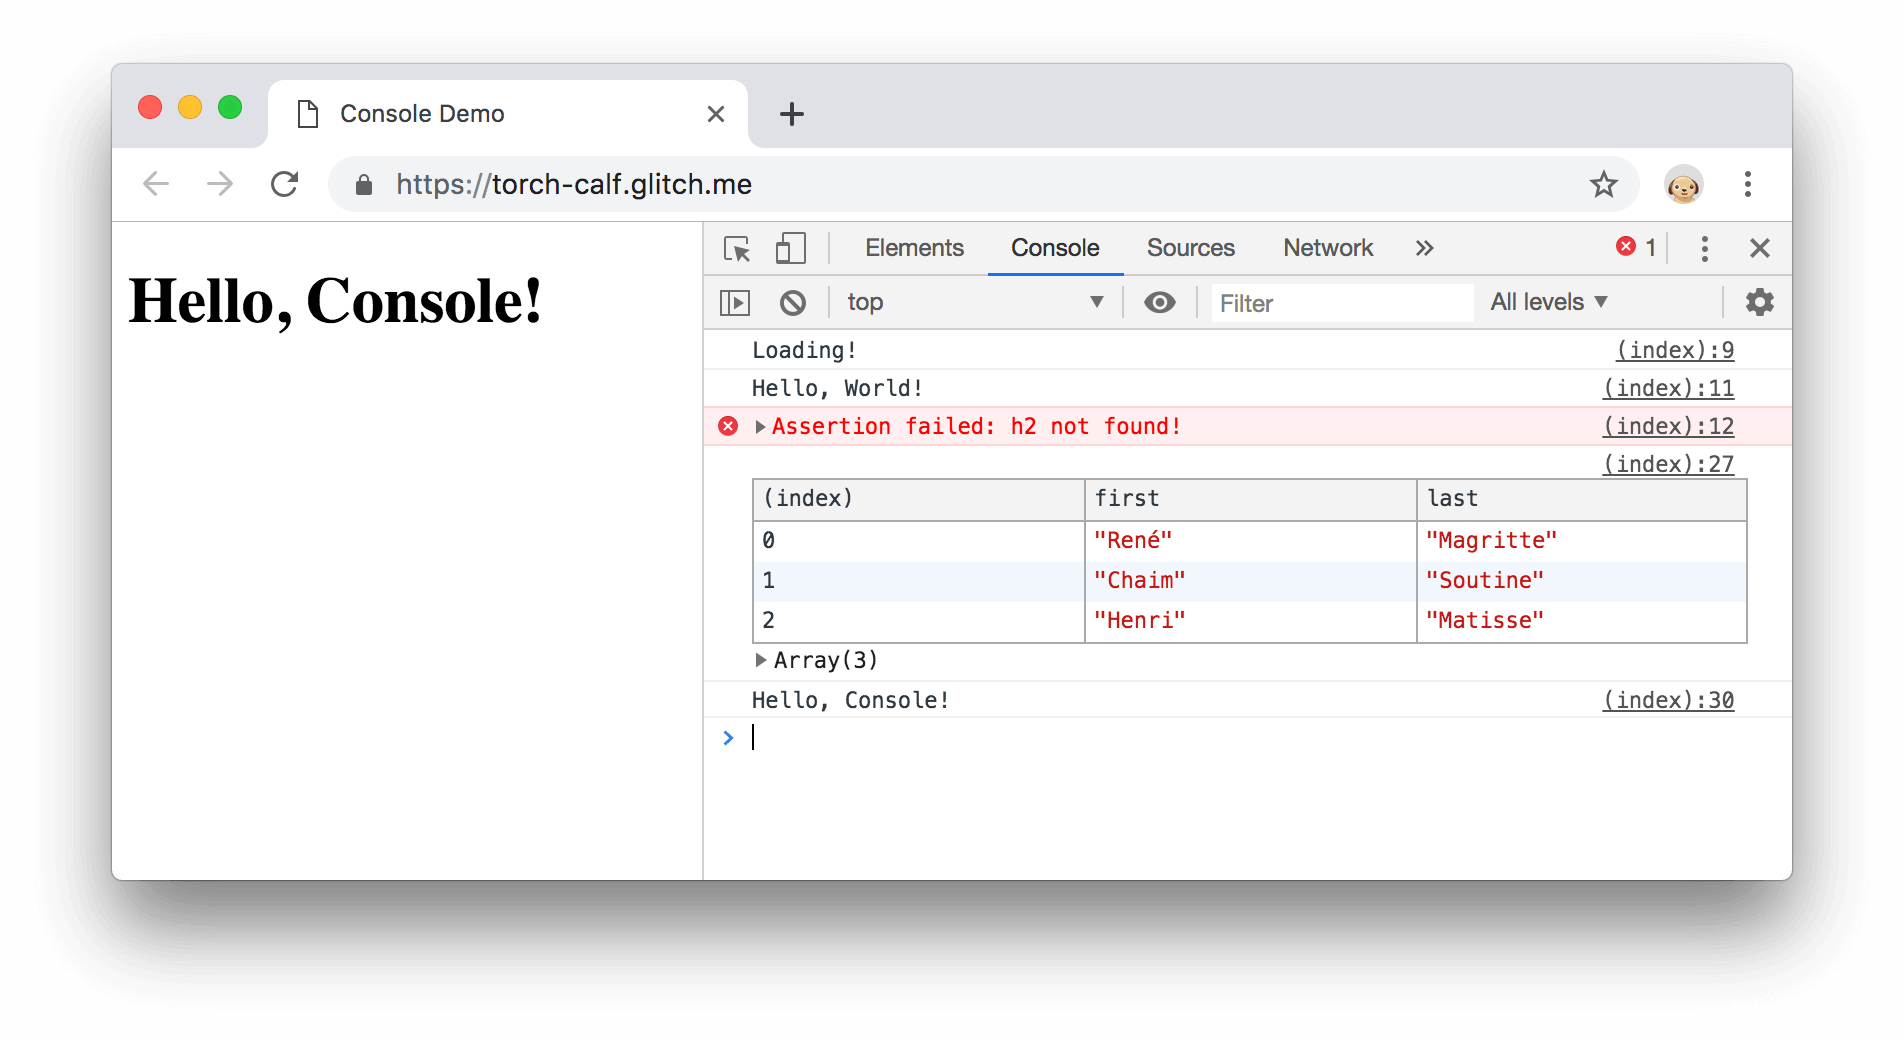
\includegraphics[width=0.9\linewidth]{console_panel.png}
  \caption{Chrome 浏览器的控制台界面(英文) \cite{chromeconsole}}
  \label{fig:console}
\end{figure}

\subsection{展示运动的频域}

在节 \ref{sec:theory_fft} 中提到,
我们需要分析运动的频域.
因为振动的频域通常是离散而稀疏的,
而且高频区域通常是几乎为零的,
所以最好将低频区域沿着屏幕的宽度延展,
然后将相邻的频域图像上的点用线段连接起来.

因为rpg\_core.js不带有在\mintinline{js}{Bitmap}对象上画直线的方法,
所以我们需要实现画直线的算法.
本模拟器采用Bresenham的直线算法.

\section{操作指南}
\label{sec:program}

当用户打开\href{https://UlyssesZh.github.io/rpg/mechsimul2}{网页},
模拟器会开始模拟默认的模型,
这是带有交变外力\cite[p. 61]{landau1976mechanics}的一维参变振动\cite[p. 82]{landau1976mechanics}
\begin{equation}
  \mathcal H\left(t,q,p\right)=\frac{p^2}2+\omega^2\left(1+u\cos\left(\gamma t\right)\right)\frac{q^2}2-fq\cos\left(\kappa t+\beta\right),
\end{equation}
其中
\begin{equation*}
  \left(u,\gamma,\beta,\kappa,\omega,f\right)=\left(0.3,21.7,0.2,8,10,20\right),
\end{equation*}
初条件为
\begin{equation*}
  \left(q,p\right)=\left(2,0\right).
\end{equation*}

\begin{figure}[h]
  \centering
  \begin{subfigure}[b]{0.45\linewidth}
    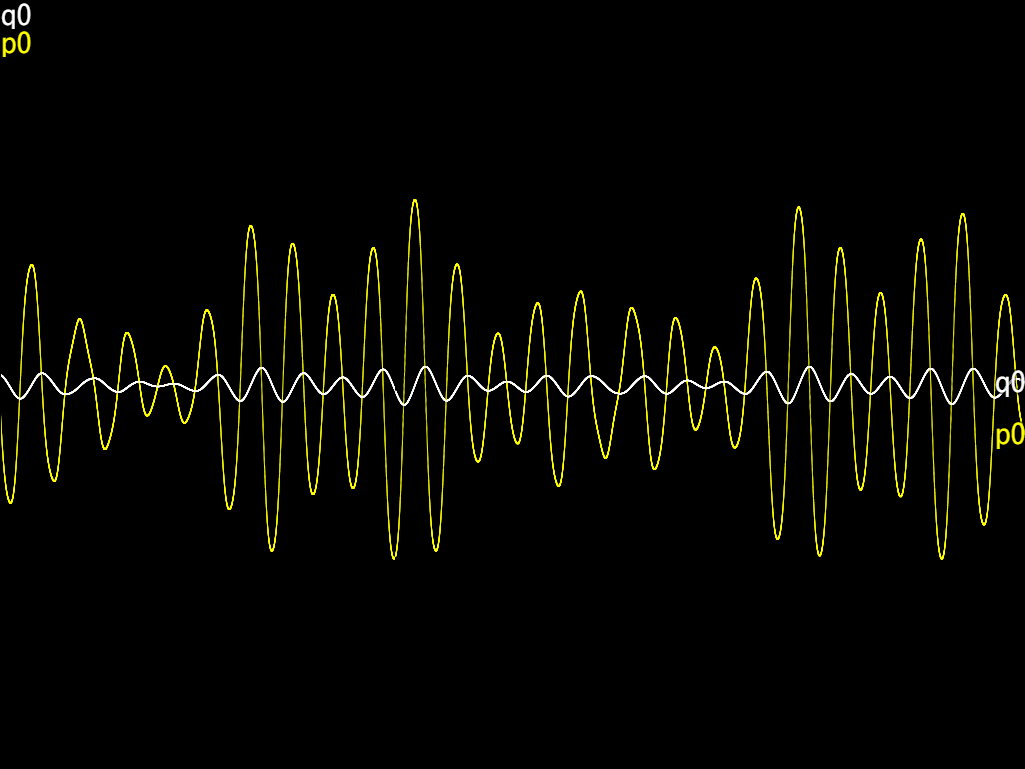
\includegraphics[width=\linewidth]{default_motion.png}
    \caption{默认模型模拟出的运动}
  \end{subfigure}
  \begin{subfigure}[b]{0.45\linewidth}
    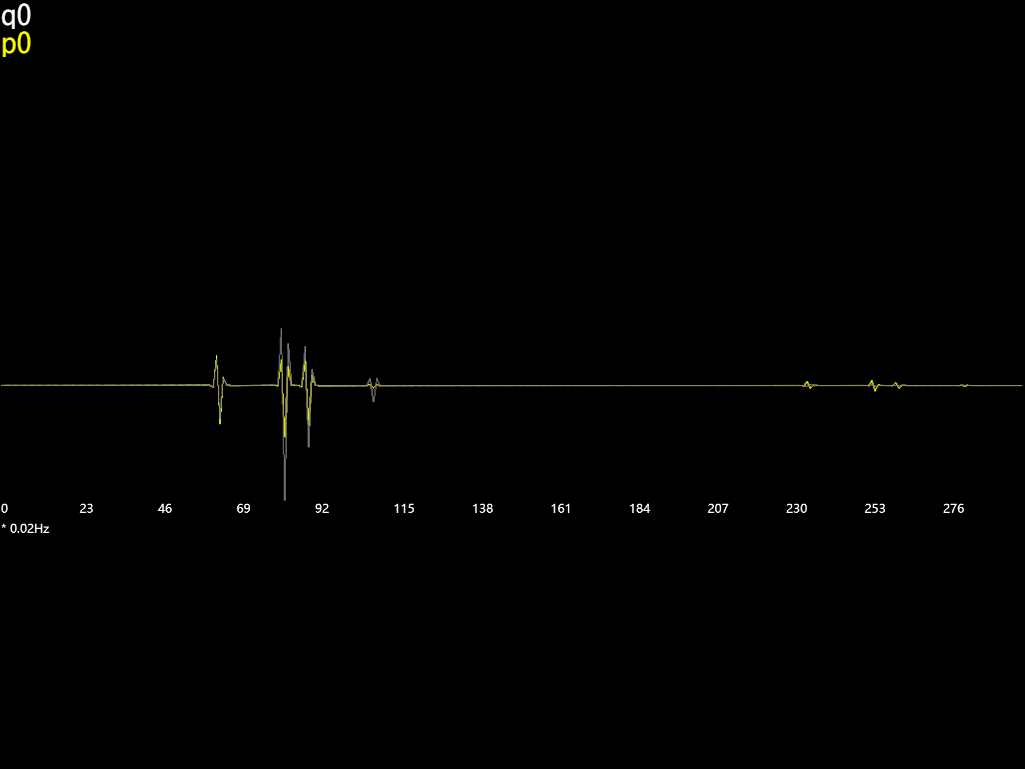
\includegraphics[width=\linewidth]{default_p0_frequencies.png}
    \caption{默认模型中$p$的频域}
  \end{subfigure}
  \caption{模拟器模拟默认模型的截屏}
  \label{fig:default}
\end{figure}

频域计算功能被启用.
一段时间后,当积累了足够多的样本,
模拟器会在屏幕左上角创建按钮,
点击按钮可以让模拟器显示将被FFT的函数时域以及计算出的频域结果.

在频域的界面,
和按钮颜色相同的线表征FFT结果的实部,
灰色的线表征FFT结果的虚部.

按\LKeySpace 以暂停或继续模拟.

图 \ref{fig:default} 展示了模拟器的图形界面.
从模拟结果看,
我们确实能学到一些运动规律.
频域图像很清晰.

如节 \ref{sec:intro} 中所介绍,模拟器可以被高度自定义.
用户能通过在控制台\footnote{
  对于大多数模拟器,按\LKeyF{12}以打开控制台.
  控制台的界面通常像图 \ref{fig:console}.
}运行代码来自定义模拟器.

\subsection{下载运动数据}

模拟器默认不会记录ODE求解器的历史.
为了让模拟器记录历史,需要运行下面的代码.

\begin{minted}{js}
  rungeKutta.recordHistory = true;
  restart();
\end{minted}

等待ODE求解器积累足够的数据,
然后运行下面的代码来下载模拟出的数据.

\begin{minted}{js}
  rungeKutta.downloadHistory(0, 30);
\end{minted}

用户需要将\mintinline{js}{0}和\mintinline{js}{30}替换为想要下载的被模拟出的数据的时间的区间端点.
如果省略这两个参数,模拟器会下载目前模拟出的所有数据.

\subsection{改变默认模型的参数}

可以通过简单的代码改变参数.
以研究参变共振的规律为例.
对于一个参变振动模型,当$\gamma\approx2\omega$时,
它达到参变共振的条件是\footnote{
  精确到$\mathrm O\left(u\right)$.
} \cite[p. 82]{landau1976mechanics}
\begin{equation}
  \left|\gamma-2\omega\right|<\frac12\omega u.
\end{equation}

用户想要研究当它达到参变共振时运动的样子,
可以令$f:=0$来取消交变外力,
并令$\gamma:=21.3$来使系统满足参变共振的条件.
然后,运行\mintinline{js}{restart()}.

\begin{minted}{js}
  f = 0;
  gamma = 21.3;
  restart();
\end{minted}

\subsection{改变初条件}

初条件$\mathbf x\left(0\right)$可以通过运行下面的代码自定义.

\begin{minted}{js}
  rungeKutta.initial = [2, 0];
  restart();
\end{minted}

将\mintinline{js}{[2, 0]}改为任意想要的初条件.

\subsection{改变尺度}

该模拟器可以改变绘制图像的尺度.
例如,对参变共振模型的模拟结果如图 \ref{fig:parametric_a} 所示.
可以发现,振幅确实如理论预言般指数增长,因而图像很快超出了屏幕范围.
我们可以使用对数尺度来避免这一点.
这可以通过用下面的代码改变$m_y$来完成.

\begin{minted}{js}
  canvas.mappingY = y => 20 * log1p(abs(y)) * sign(y) + Graphics.height/2;
  restart();
\end{minted}

现在$m_y\left(y\right):=20\ln\left(1+\left|y\right|\right)\operatorname{sgn}y+h/2$.

注意,在代码中\mintinline{js}{Graphics.width}代表$w$,
\mintinline{js}{Graphics.height}代表$h$.

参变共振的模拟结果可以在图 \ref{fig:parametric} 中被看到.
可以看到振幅确实在按指数增加.

\begin{figure}[h]
  \centering
  \begin{subfigure}[b]{0.45\linewidth}
    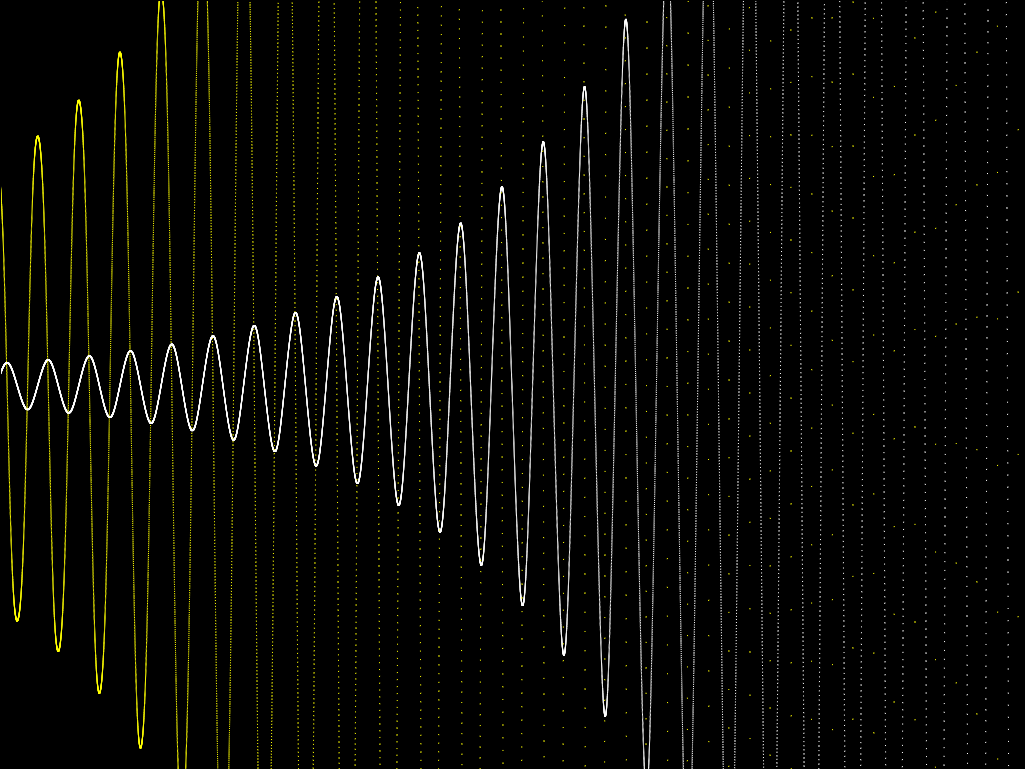
\includegraphics[width=\linewidth]{parametric_resonance.png}
    \caption{参变共振现象被模拟}
    \label{fig:parametric_a}
  \end{subfigure}
  \begin{subfigure}[b]{0.45\linewidth}
    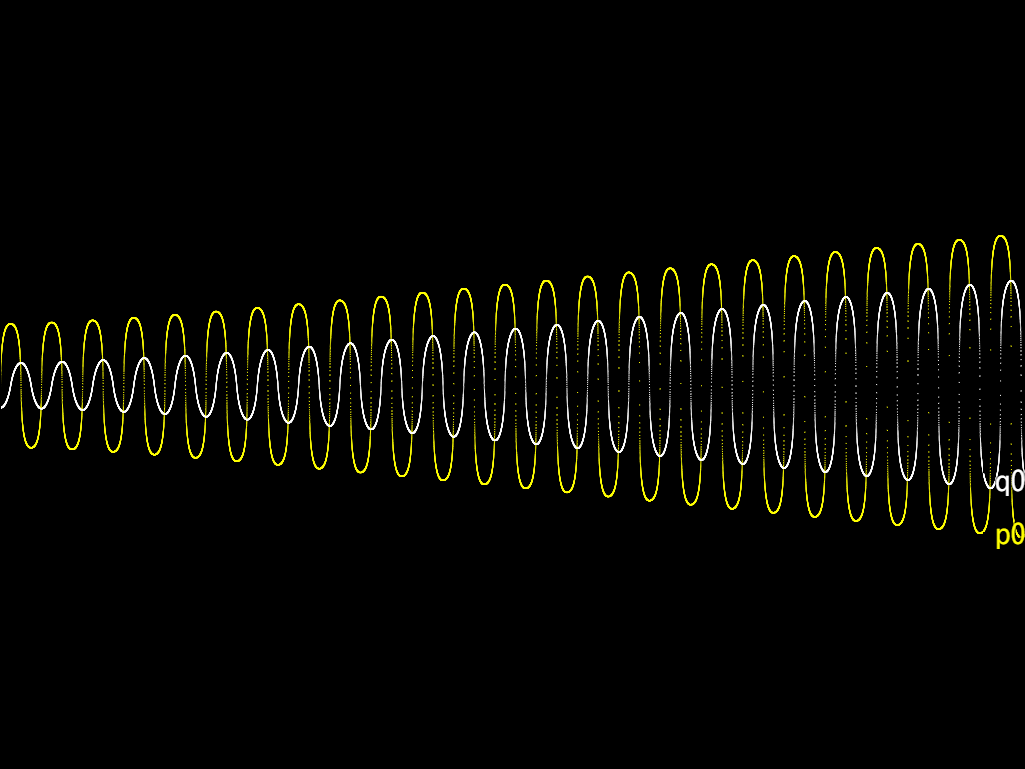
\includegraphics[width=\linewidth]{parametric_resonance_logarithmic.png}
    \caption{使用对数尺度防止振幅增长过快}
    \label{fig:parametric_b}
  \end{subfigure}
  \caption{模拟器模拟参变共振}
  \label{fig:parametric}
\end{figure}

\subsection{关闭频域分析}

用户能通过下面的代码关闭频域分析.
运行该代码后,左上角不会再出现表明频域已准备好的按钮.

\begin{minted}{js}
  canvas.detectPeriod = false;
  restart();
\end{minted}

\subsection{高级:绘制相图}

相图是表示相点$\mathbf x$的运动的图像\cite[p. 146]{landau1976mechanics}\cite[p. 68]{arnold1989mathmech}.

该模拟器带有允许用户在ODE求解器推进时运行自定义代码的API.
为了绘制相图,首先用户需要用下面的代码创建\mintinline{js}{Sprite}对象和\mintinline{js}{Bitmap}对象.

\begin{minted}{js}
  var phaseSprite = new Sprite();
  phaseSprite.bitmap = new Bitmap(Graphics.width, Graphics.height);
  scene.addChild(phaseSprite);
\end{minted}

然后,改变\mintinline{js}{canvas.onTrace},用于当新的点被添加时运行自定义代码,
并\mintinline{js}{restart()}.

\begin{minted}{js}
  canvas.onTrace = (t, qp) => {
    phaseSprite.bitmap.setPixel(...qp.map(canvas.mappingY), 'white');
    return true;
  };
  restart();
\end{minted}

用户还可以通过运行\mintinline{js}{canvas.visible = false;}来隐藏原始画布.

也能在任何时候通过运行\mintinline{js}{phaseSprite.bitmap.clear();}来清空相图.

\begin{figure}
  \centering
  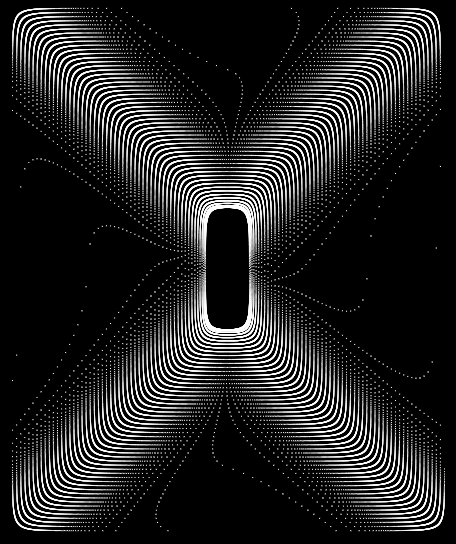
\includegraphics[width=0.3\linewidth]{parametric_resonance_logarithmic_phase.png}
  \caption{对数尺度下参变共振运动的相图}
  \label{fig:parametric_phase}
\end{figure}

图 \ref{fig:parametric_phase} 展示了上面的代码的运行结果.

每个周期的相图的边上的线应当是连续的,
但是因为相点移动得过快,模拟器不能连续地追踪它.
这些离散的点看似在相图中形成了曲线,
可以在图 \ref{fig:parametric_phase} 中看出来.
这些曲线的方程是什么?
看来使用该模拟器还能启发我们研究这样的问题
并鼓励我们学习一些像这样的有关物理的东西.

\subsection{将当前模型的Hamiltonian改成非线性振子的Hamiltonian}

\begin{figure}
  \centering
  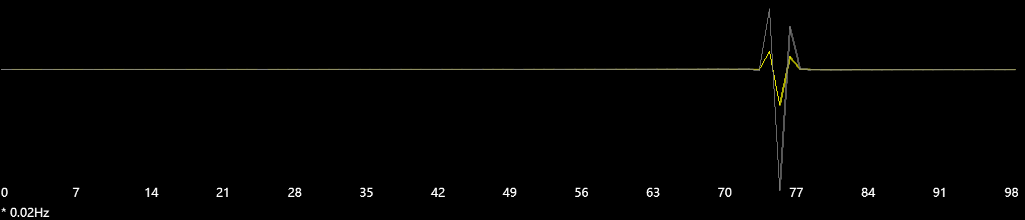
\includegraphics[width=0.9\linewidth]{nonlinear_frequency.png}
  \caption{非线性振子的频域(高频区域没有显示)}
  \label{fig:nonlinear}
\end{figure}

用户可以将一个函数赋值给变量\mintinline{js}{rungeKutta.func}
来改变式 \ref{eq:ode} 中的$\mathbf f$.
为了按照式 \ref{eq:def_f} 根据Hamiltonian创建$\mathbf f$,
使用函数\mintinline{js}{canonicalEquation},
其第一个参数为DOF,第二个参数为Hamiltonian函数.

一个例子是将默认模型的Hamiltonian改为非线性振子的
\begin{equation*}
  \mathcal H\left(t,q,p\right):=\frac{p^2}2+\frac{\omega_0^2q^2}2+\alpha q^3+\beta q^4,
\end{equation*}
可以通过运行下面的代码实现.
在使用该代码前,需要刷新网页\footnote{
  对于大多数浏览器,刷新的快捷键是\LKeyF{5}.
}以获得清洁的环境,防止对前一个模型的更改继续产生效果.

\begin{minted}{js}
  rungeKutta.func = canonicalEquation(1, (t, qp) => {
    let [q, p] = qp;
    return p**2/2 + omega0**2*q**2/2 + alpha*q**3 + beta*q**4;
  });
\end{minted}

接下来需要定义参数$\left(\omega_0,\alpha,\beta\right)$和设置初条件.
假设取
\begin{equation*}
  \left(\omega_0,\alpha,\beta\right):=\left(10,-2,-3\right),
\end{equation*}
运行如下代码.

\begin{minted}{js}
  var omega0 = 10;
  var alpha = -2;
  var beta = -3;
\end{minted}

假设取初条件$\left(q,p\right)=\left(1,0\right)$, 即振幅被设定为$b=1$, 运行如下代码.

\begin{minted}{js}
  rungeKutta.initial = [1, 0];
\end{minted}

我们可以用模拟器验证计算非线性振子的振动频率的公式\cite[p. 87]{landau1976mechanics}\footnote{
  精确到$\mathrm O\left(b^2\right)$.
}
\begin{equation*}
  \omega=\omega_0+\left(\frac{3\beta}{2\omega_0}-\frac{15\alpha^2}{4\omega_0^3}\right)b^2=9.535.
\end{equation*}

其频域在图 \ref{fig:nonlinear} 中展示.
可以看到,频率大约是理论预测值$\frac\omega{2\pi}=1.518$,
与线性振子的频率$\frac{\omega_0}{2\pi}=1.592$不同.

\section{案例}
\label{sec:examples}

在节 \ref{sec:program} 呈现的默认模型以及对默认模型的典型的自定义都是该模拟器的很好的应用案例.

除此以外,本节将介绍一些其他的应用案例.
这些案例的代码都可以在\href{https://ulysseszh.github.io/rpg/mechsimul2/examples.html}{网页}上找到.

\subsection{Kepler二体问题}

二体问题是具有$4$ DOF的系统.
将被模拟的模型的Hamiltonian是
\begin{equation*}
  \mathcal H\left(t,q_0,q_1,q_2,q_3,p_0,p_1,p_2,p_3\right):=
  p_0^2+p_1^2+p_2^3+p_3^2-\frac{500}{\sqrt{\left(q_0-q_2\right)^2+\left(q_1-q_3\right)^2}}.
\end{equation*}

\begin{figure}[h]
  \centering
  \begin{subfigure}[b]{0.6\linewidth}
    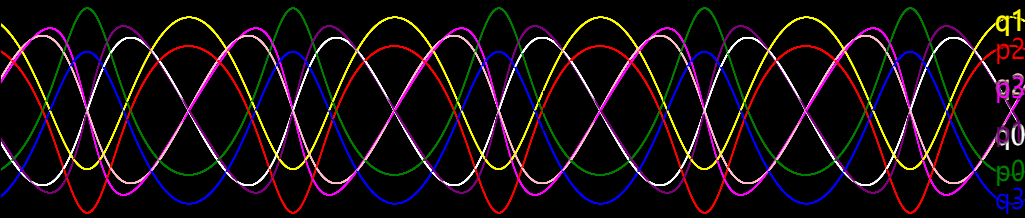
\includegraphics[width=\linewidth]{kepler_2_body_graph.png}
    \caption{$\mathbf x$的图像,共8条曲线}
  \end{subfigure}
  \begin{subfigure}[b]{0.15\linewidth}
    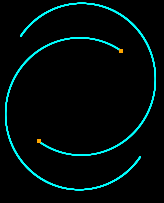
\includegraphics[width=\linewidth]{kepler_2_body_trace.png}
    \caption{可视化}
  \end{subfigure}
  \begin{subfigure}[b]{0.2\linewidth}
    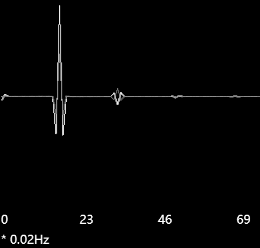
\includegraphics[width=\linewidth]{kepler_2_body_q0_frequencies.png}
    \caption{$q_0$的频域}
  \end{subfigure}
  \caption{模拟器模拟Kepler二体问题}
  \label{fig:kepler}
\end{figure}

运行下面的代码,然后会得到两个互相运动的恒星.

\begin{minted}{js}
  // 画布上有 8 条曲线将被绘制
  canvas.n = 8;
  // 设置系统的 Hamiltonian
  rungeKutta.func = canonicalEquation(4, (t, qp) => {
    let [x1, y1, x2, y2, px1, py1, px2, py2] = qp;
    return px1**2 + py1**2 + px2**2 + py2**2 - 500 / hypot(x1-x2, y1-y2);
  });
  // 设置系统的初条件
  rungeKutta.initial = [-3, -3, 3, 3, 2, -3, -2, 3];
  // 设置图像的尺度
  canvas.mappingY = y => 20 * y + Graphics.height/2;
  // 设置图像的颜色. 有 8 条曲线, 所以设置 8 个颜色
  canvas.colors = ["white", "yellow", "pink", "blue",
                   "green", "purple", "red", "magenta"];

  // 下面的代码创建用于可视化的 Sprite 对象和 Bitmap 对象
  // 使用 rpg_core.js 提供的 API, 见 [1] 获取帮助
  var traceSprite = new Sprite();
  var star1 = new Sprite();
  var star2 = new Sprite();
  scene.addChild(traceSprite);
  scene.addChild(star1);
  scene.addChild(star2);
  traceSprite.bitmap = new Bitmap(Graphics.width, Graphics.height);
  star1.bitmap = star2.bitmap = new Bitmap(4, 4);
  star1.bitmap.fillAll('orange');
  star1.anchor.x = star1.anchor.y = 0.5;
  star2.anchor.x = star2.anchor.y = 0.5;

  // 当新的样本出现时, 更新 Sprite 对象的状态
  canvas.onTrace = (t, qp) => {
    // 设置恒星的 Sprite 对象的位置
    [star1.x, star1.y, star2.x, star2.y] =
        qp.slice(0, 4).map(canvas.mappingY);
    // 描出轨迹
    traceSprite.bitmap.setPixel(star1.x, star1.y, 'cyan');
    traceSprite.bitmap.setPixel(star2.x, star2.y, 'cyan');
    return true;
  };

  // 重新开始以应用改变
  restart();
\end{minted}

模拟出的结果在图 \ref{fig:kepler} 中展示.

如果用户好奇, Hamiltonian或初条件可以被修改以创建有趣的图像.

行\mintinline{js}{rungeKutta.initial = [-3, -3, 3, 3, 5, -2, -5, 2];}
可以被修改以应用不同的初条件.
对于不同的初条件,轨迹能呈现不同的形状.
如果把\mintinline{js}{2, -3, -2, 3}换成\mintinline{js}{5, -2, -5, 2},
轨迹是如图 \ref{fig:distortion_kepler} 所示的双曲线.

行\mintinline{js}{return px1**2 + py1**2 + px2**2 + py2**2 - 500 / hypot(x1-x2, y1-y2);}
可以被更改以给系统应用一个不同的Hamiltonian.
如果将\mintinline{js}{x1-x2}变为\mintinline{js}{1.5*x1-x2},
得到的是如图 \ref{fig:distortion_kepler} 所示的混乱的运动.

\begin{figure}[h]
  \centering
  \begin{subfigure}[b]{0.4\linewidth}
    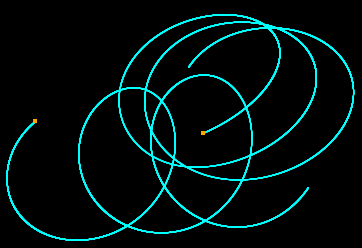
\includegraphics[width=\linewidth]{distortion_kepler.png}
    \caption{代码\mintinline{js}{x1-x2}变为\mintinline{js}{1.5*x1-x2}}
  \end{subfigure}
  \begin{subfigure}[b]{0.4\linewidth}
    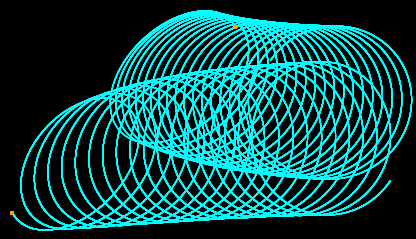
\includegraphics[width=\linewidth]{distortion2_kepler.png}
    \caption{代码\mintinline{js}{x1-x2}变为\mintinline{js}{1.1*x1-x2}}
  \end{subfigure}
  \begin{subfigure}[b]{0.6\linewidth}
    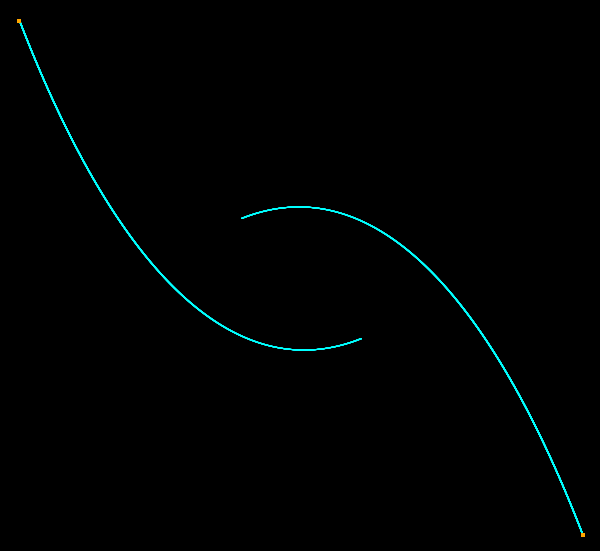
\includegraphics[width=\linewidth]{distortion3_kepler.png}
    \caption{代码\mintinline{js}{2, -3, -2, 3}变为\mintinline{js}{5, -2, -5, 2}}
  \end{subfigure}
  \caption{Kepler二体问题模型被更改}
  \label{fig:distortion_kepler}
\end{figure}

\subsection{浸渐不变量}

一维周期运动的作用变量是浸渐不变量,
它在Hamiltonian中的参数缓慢变化时保持不变\cite[p. 298]{arnold1989mathmech}\cite[p. 156]{landau1976mechanics}.

一个与浸渐不变量有关的系统有些难以想象.
我们想要用模拟器展示浸渐不变量如何起作用.
下面展示的代码能够被修改以模拟其他与浸渐不变量有关的系统.

这里被采用的案例是频率缓慢变化的简谐振子.
它的Hamiltonian是
\begin{equation*}
  \mathcal H\left(t,q,p\right)=\frac{p^2}2+\omega\left(t\right)^2\frac{q^2}2,
\end{equation*}
其中$\omega\left(t\right):=4+0.05t$关于$t$缓慢变化.

根据作用变量的定义,
可以得到简谐振子的浸渐不变量为\cite[p. 300]{arnold1989mathmech}\cite[p. 157]{landau1976mechanics}
\begin{equation*}
  I=\frac{\mathcal H}\omega.
\end{equation*}

通过运行下面的代码把$I$和$\mathcal H$的图像绘制在画布上.

\begin{minted}{js}
  // 上面提到的变化参数 omega. 它应当缓慢变化
  var omega = t => 4 + 0.05 * t;
  // 系统的 Hamiltonian
  var hamiltonian = (t, qp) => qp[1]**2/2 + omega(t)**2 * qp[0]**2/2;
  // 设置系统的 Hamiltonian
  rungeKutta.func = canonicalEquation(1, hamiltonian);
  // 有 4 条曲线需要在画布上被绘制
  canvas.n = 4;
  // 曲线的标签将会是 q, p, H, I
  canvas.getLabelString = i => 'qpHI'[i];
  // 曲线的颜色
  canvas.colors = ["white", "yellow", "pink", "blue"];
  // 当新的样本产生时跟踪 I 和 H
  canvas.trace = function (t, data) {
    // 计算此时的 Hamiltonian 值
    let h = hamiltonian(t, data);
    // 此时要在画布上画的内容: [q, p, h, h/omega]
    data = data.concat([h, h / omega(t)]);
    // 调用旧方法, 这是 JavaScript 的技巧
    return this.__proto__.trace.call(this, t, data);
  };
  // 重新开始以应用改变
  restart();
\end{minted}

上面代码的注释标记了缓变参数和Hamiltonian的定义.
可以随意地改变它们来模拟其他有浸渐不变量的系统.

\begin{figure}[h]
  \centering
  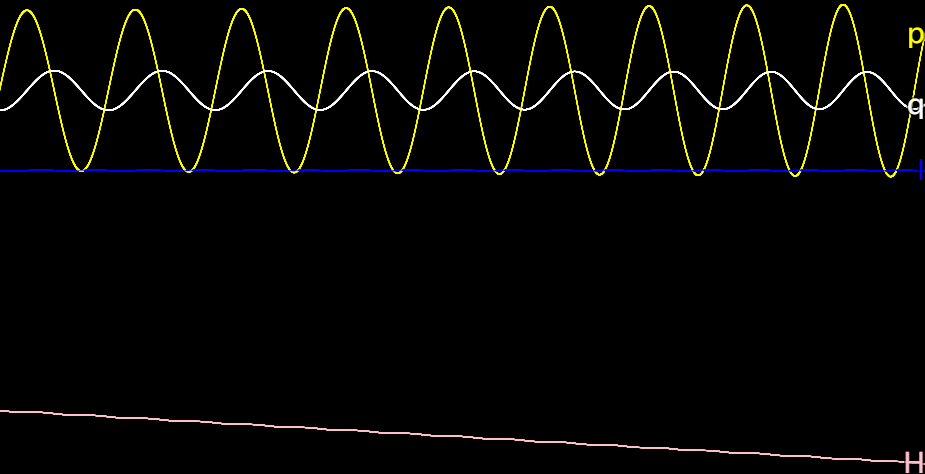
\includegraphics[width=0.6\linewidth]{adiabatic.png}
  \caption{带有缓变参数的简谐振子的浸渐不变量}
  \label{fig:adiabatic}
\end{figure}

图 \ref{fig:adiabatic} 展示了结果.
可以看到,当$\omega$以及$\mathcal H$缓变, $I$不变,与理论预言相同.

\subsection{粒子束散射}

假设有一束全同粒子向有心力场发射,
粒子束的每个粒子具有Hamiltonian
\begin{equation*}
  \mathcal H\left(t,q_0,q_1,p_0,p_1\right)=p_0^2+p_1^2+\frac{30}{\sqrt{q_0^2+q_1^2}}.
\end{equation*}

粒子束会被散射,具有不同的瞄准距离的粒子会有不同的散射角\cite[p. 49]{landau1976mechanics}.
我们想要用模拟器研究这一现象.

可以用下面的代码完成这一模拟.
注意,在低配置设备上,模拟较为缓慢,
因为同时有30个运动被模拟.

\begin{minted}{js}
  // 粒子束中的粒子总数
  var n = 30;
  // n 个 ODE 求解器的数组
  rungeKuttas = [];
  for (let i = 0; i < n; i++) {
    // 创建 ODE 求解器
    rungeKuttas[i] = RungeKutta.solveHamiltonian(
      // 参数列表:
      2,                           // 自由度
      [-20, (i - n/2)*0.3, 4, 0],  // 初条件
      Number.POSITIVE_INFINITY,    // 模拟的最长时间
      null,                        // 画布. null 表示无画布
      (t, qp) => {                 // Hamiltonian
        let [x, y, px, py] = qp;
        return px**2 + py**2 + 30/hypot(x,y);
      }
    );
  }

  // 创建用于可视化的 Sprite 对象和 Bitmap 对象 (rpg_core.js API)
  var traceSprite = new Sprite();
  scene.addChild(traceSprite);
  traceSprite.bitmap = new Bitmap(Graphics.width, Graphics.height);

  // 绘图的尺度
  var my = y => 20 * y + Graphics.height/2;
  // 每帧更新时调用的函数
  update = function () {
    for (let i = 0; i < n; i++) {
      // 计算描点坐标
      let xy = [0, 1].map(j => my(rungeKuttas[i].current[j]))
      // 描出轨迹上的点
      traceSprite.bitmap.setPixel(...xy, 'white');
      // ODE 求解器推进
      rungeKuttas[i].update();
    }
  };

  // 重新开始以应用更改
  restart();
  // 隐藏原始画布
  canvas.visible = false;
\end{minted}

\begin{figure}[h]
  \centering
  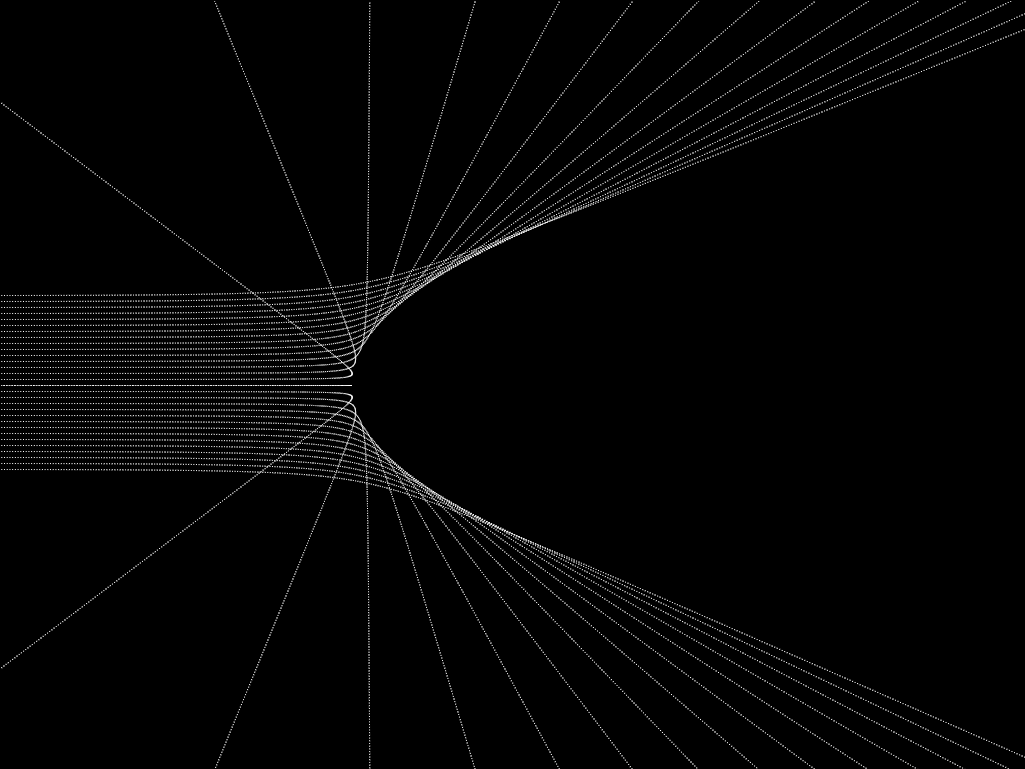
\includegraphics[width=0.8\linewidth]{scatter.png}
  \caption{被散射的粒子的轨迹}
  \label{fig:scatter}
\end{figure}

\begin{figure}[h]
  \centering
  \begin{subfigure}[b]{0.4\linewidth}
    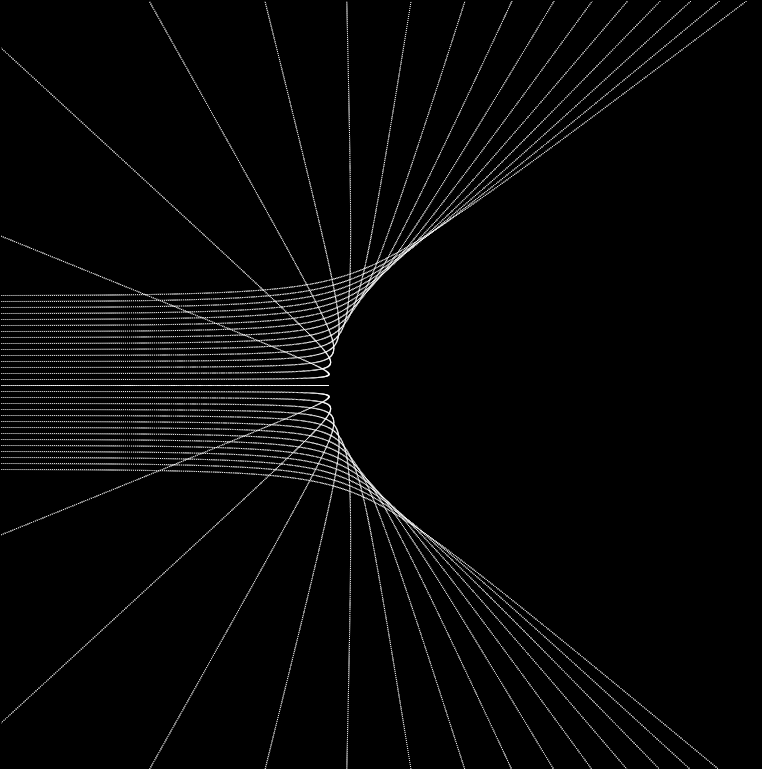
\includegraphics[width=\linewidth]{distortion_scatter.png}
    \caption{代码\mintinline{js}{4, 0}变为\mintinline{js}{3, 0},轨迹更加弯曲}
  \end{subfigure}
  \begin{subfigure}[b]{0.5\linewidth}
    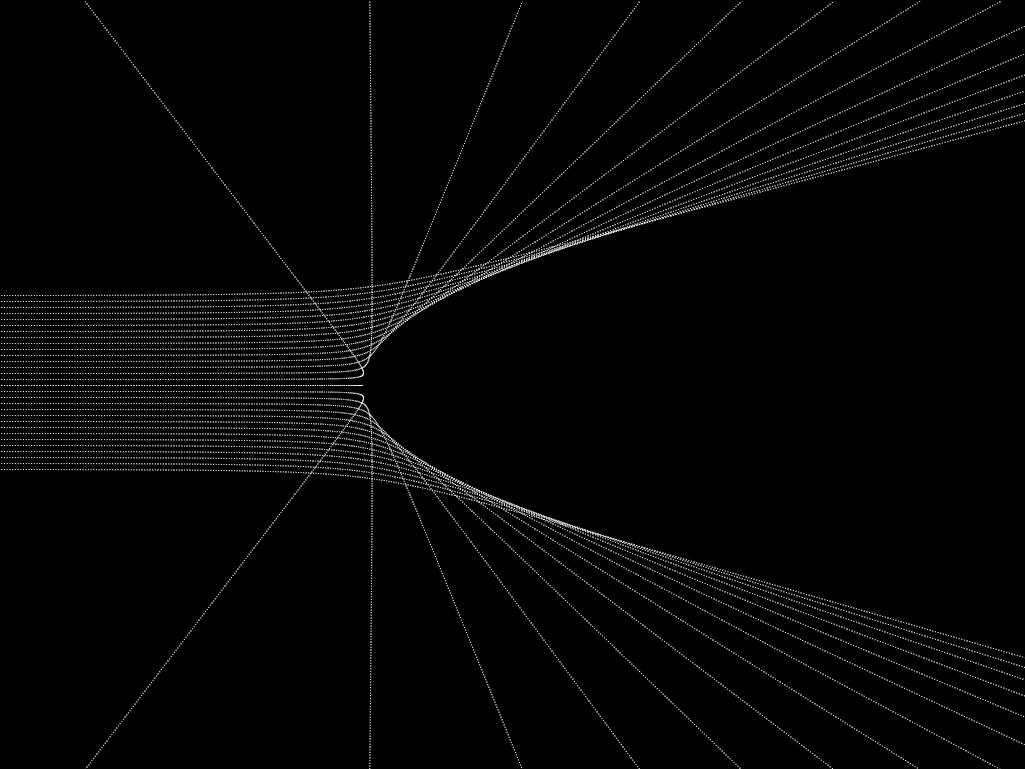
\includegraphics[width=\linewidth]{distortion2_scatter.png}
    \caption{代码\mintinline{js}{30/hypot(x,y)}变为\mintinline{js}{20/hypot(x,y)},轨迹更加平直}
  \end{subfigure}
  \caption{粒子束散射模型的参数被改变}
  \label{fig:distortion_scatter}
\end{figure}

上面的代码的结果如图 \ref{fig:scatter} 所示.

散射的效应形成了优美的图像.
可以看到,粒子的轨道的包络线看上去像是圆锥曲线.
然后,我们可以对包络线的方程是什么感到好奇,
因为它是有意义的,
它表征了粒子无法到达的区域.

像这样直观的模拟启发我们研究物理.
这正是该模拟器的好处之一.

还能研究粒子束的初始速度和场强对轨迹的影响.
我们可以用模拟器验证,当初始速度减小或场强增大时,轨迹会更加弯曲.

行\mintinline{js}{[-20, (i - n/2)*0.3, 4, 0],}指定了第\mintinline{js}{i}个粒子的初条件.

行\mintinline{js}{return px**2 + py**2 + 30/hypot(x,y);}指定了粒子的Hamiltonian.

我们将代码\mintinline{js}{4, 0}变为\mintinline{js}{3, 0}以使得轨迹更加弯曲,
将代码\mintinline{js}{30/hypot(x,y)}变为\mintinline{js}{20/hypot(x,y)}以使得轨迹更加平直,
见图 \ref{fig:distortion_scatter}.

\subsection{狭义相对论}

不仅仅是经典力学,该模拟器还能模拟狭义相对论力学,
因为相对论力学能用Hamilton力学描绘.
考虑相对论粒子在均匀重力场中的运动,它具有Hamiltonian\cite[p. 28]{landau2010fields}
\begin{equation*}
  \mathcal H\left(t,q,p\right):=\sqrt{p^2+10}-0.8q
\end{equation*}
和初条件$\left(q,p\right)=\left(-10,-10\right)$.

模拟的结果如图 \ref{fig:relativity} 所示.
随着$t\rightarrow\infty$,该粒子动量匀速增大,
速度越来越接近光速,
符合理论预言\cite[p. 24]{landau2010fields}.

\begin{figure}[h]
  \centering
  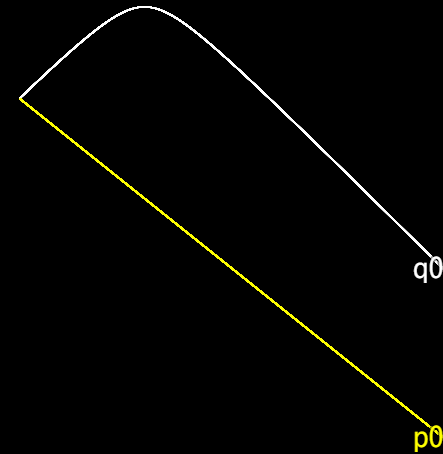
\includegraphics[width=0.25\linewidth]{relativity_gravity.png}
  \caption{均匀重力场中相对论粒子的运动}
  \label{fig:relativity}
\end{figure}

\section{结论}

我开发了一个方便的线上软件,它可以模拟Hamilton力学.
有很多能用它完成的应用案例.

该模拟器是力学模拟器.
当用户输入系统的Hamiltonian和初条件后,
模拟器能模拟系统的运动,
在屏幕上作出运动的图像.
如果振动系统被模拟,
在足够多的样本被计算出来后,
模拟器还能用FFT计算出运动的频域.

该模拟器具有以下优点:
\begin{enumerate}
  \item 体积小,速度快.
  该模拟器简单但高效.
  有良好网络环境的电脑的用户可以在没有准备的情况下在几秒内开始模拟力学系统.

  \item 非常方便.
  任何有浏览器和互联网的用户都可以在不需要下载程序文件到磁盘的情况下使用该模拟器.
  该模拟器基于HTML,程序用JavaScript写成,几乎所有浏览器都能支持.

  \item 高度可自定义.
  该模拟器的一切都可以很容易地自定义.
  被模拟的模型, ODE求解器的参数,该模拟器呈现系统的方式等等,都能自定义.

  \item 可以输出数据.
  模拟出的数据可以被输出,用于创建力学数据集.
  被创建的数据集可以用于研究系统的规律或者被第三方软件分析.

  \item 容易操作.
  用户需要做的一切就是在控制台中编写简单的JavaScript代码和点击屏幕.
  编写代码是简单的.
  如果不需要高级用法,没有编程经历的用户只需要几分钟时间就可以学会使用它.
\end{enumerate}

该模拟器可以用于研究Hamilton力学系统的运动,
学习经典理论力学,
为与物理相关的讲座或者物理课程创建动态图片,
以及创建Hamilton系统的运动的数据集.
并且非常适用于网络教学.

该模拟器带有默认模型,在节 \ref{sec:program} 中说明了它的基础应用.
在节 \ref{sec:examples} 中,介绍了一些其他的案例,用于解释一些更深远的应用.

该模拟器被挂载在\href{https://UlyssesZh.github.io/rpg/mechsimul2}{网页} (https://UlyssesZh.github.io/rpg/mechsimul2)上.

\newpage

\bibliographystyle{abbrv}
\bibliography{mechsimul}

\end{document}
